\subsection{Basic idea of subevent cumulant}
In this analysis we focus mainly on four-particle subevent cumulant, but the generalization to higher-order is straightforward. The basic idea for subevent cumulants is shown in Fig.~\ref{fig:subevt_demo}. The event is equally divided into three non-overlapping rapidity ranges, labelled as $A$, $B$ and $C$. In this analysis, $A$ is defined with $-2.5/3<\eta<2.5/3$, $B$ is defined with $-2.5<\eta<-2.5/3$ and $C$ is defined with $2.5/3<\eta<2.5$. Four-particle correlators are then constructed by choosing two particles from subevent $A$ and one particle each from subevents $B$ and $C$. All other permutations are also considered to increase the number of pairs (e.g. two particles from subevent $B$ and one particle each from subevent $A$ and $C$). Dijets contributions, the main source for non-flow, are suppressed, since they can only produce particles in each subevent. For comparison, we also consider cumulants based on two subevents as shown in Fig.~\ref{fig:subevt_demo}. In this case, two particles each are chosen from $A$ and $B$, which effectively suppress contribution from single jet, but not away-side jets when it lands in different subevents. For the 2 subevent, in this analysis, $A$ is defined with $\eta<0$ and $B$ is defined with $\eta>0$.

\begin{figure}[H]
\centering
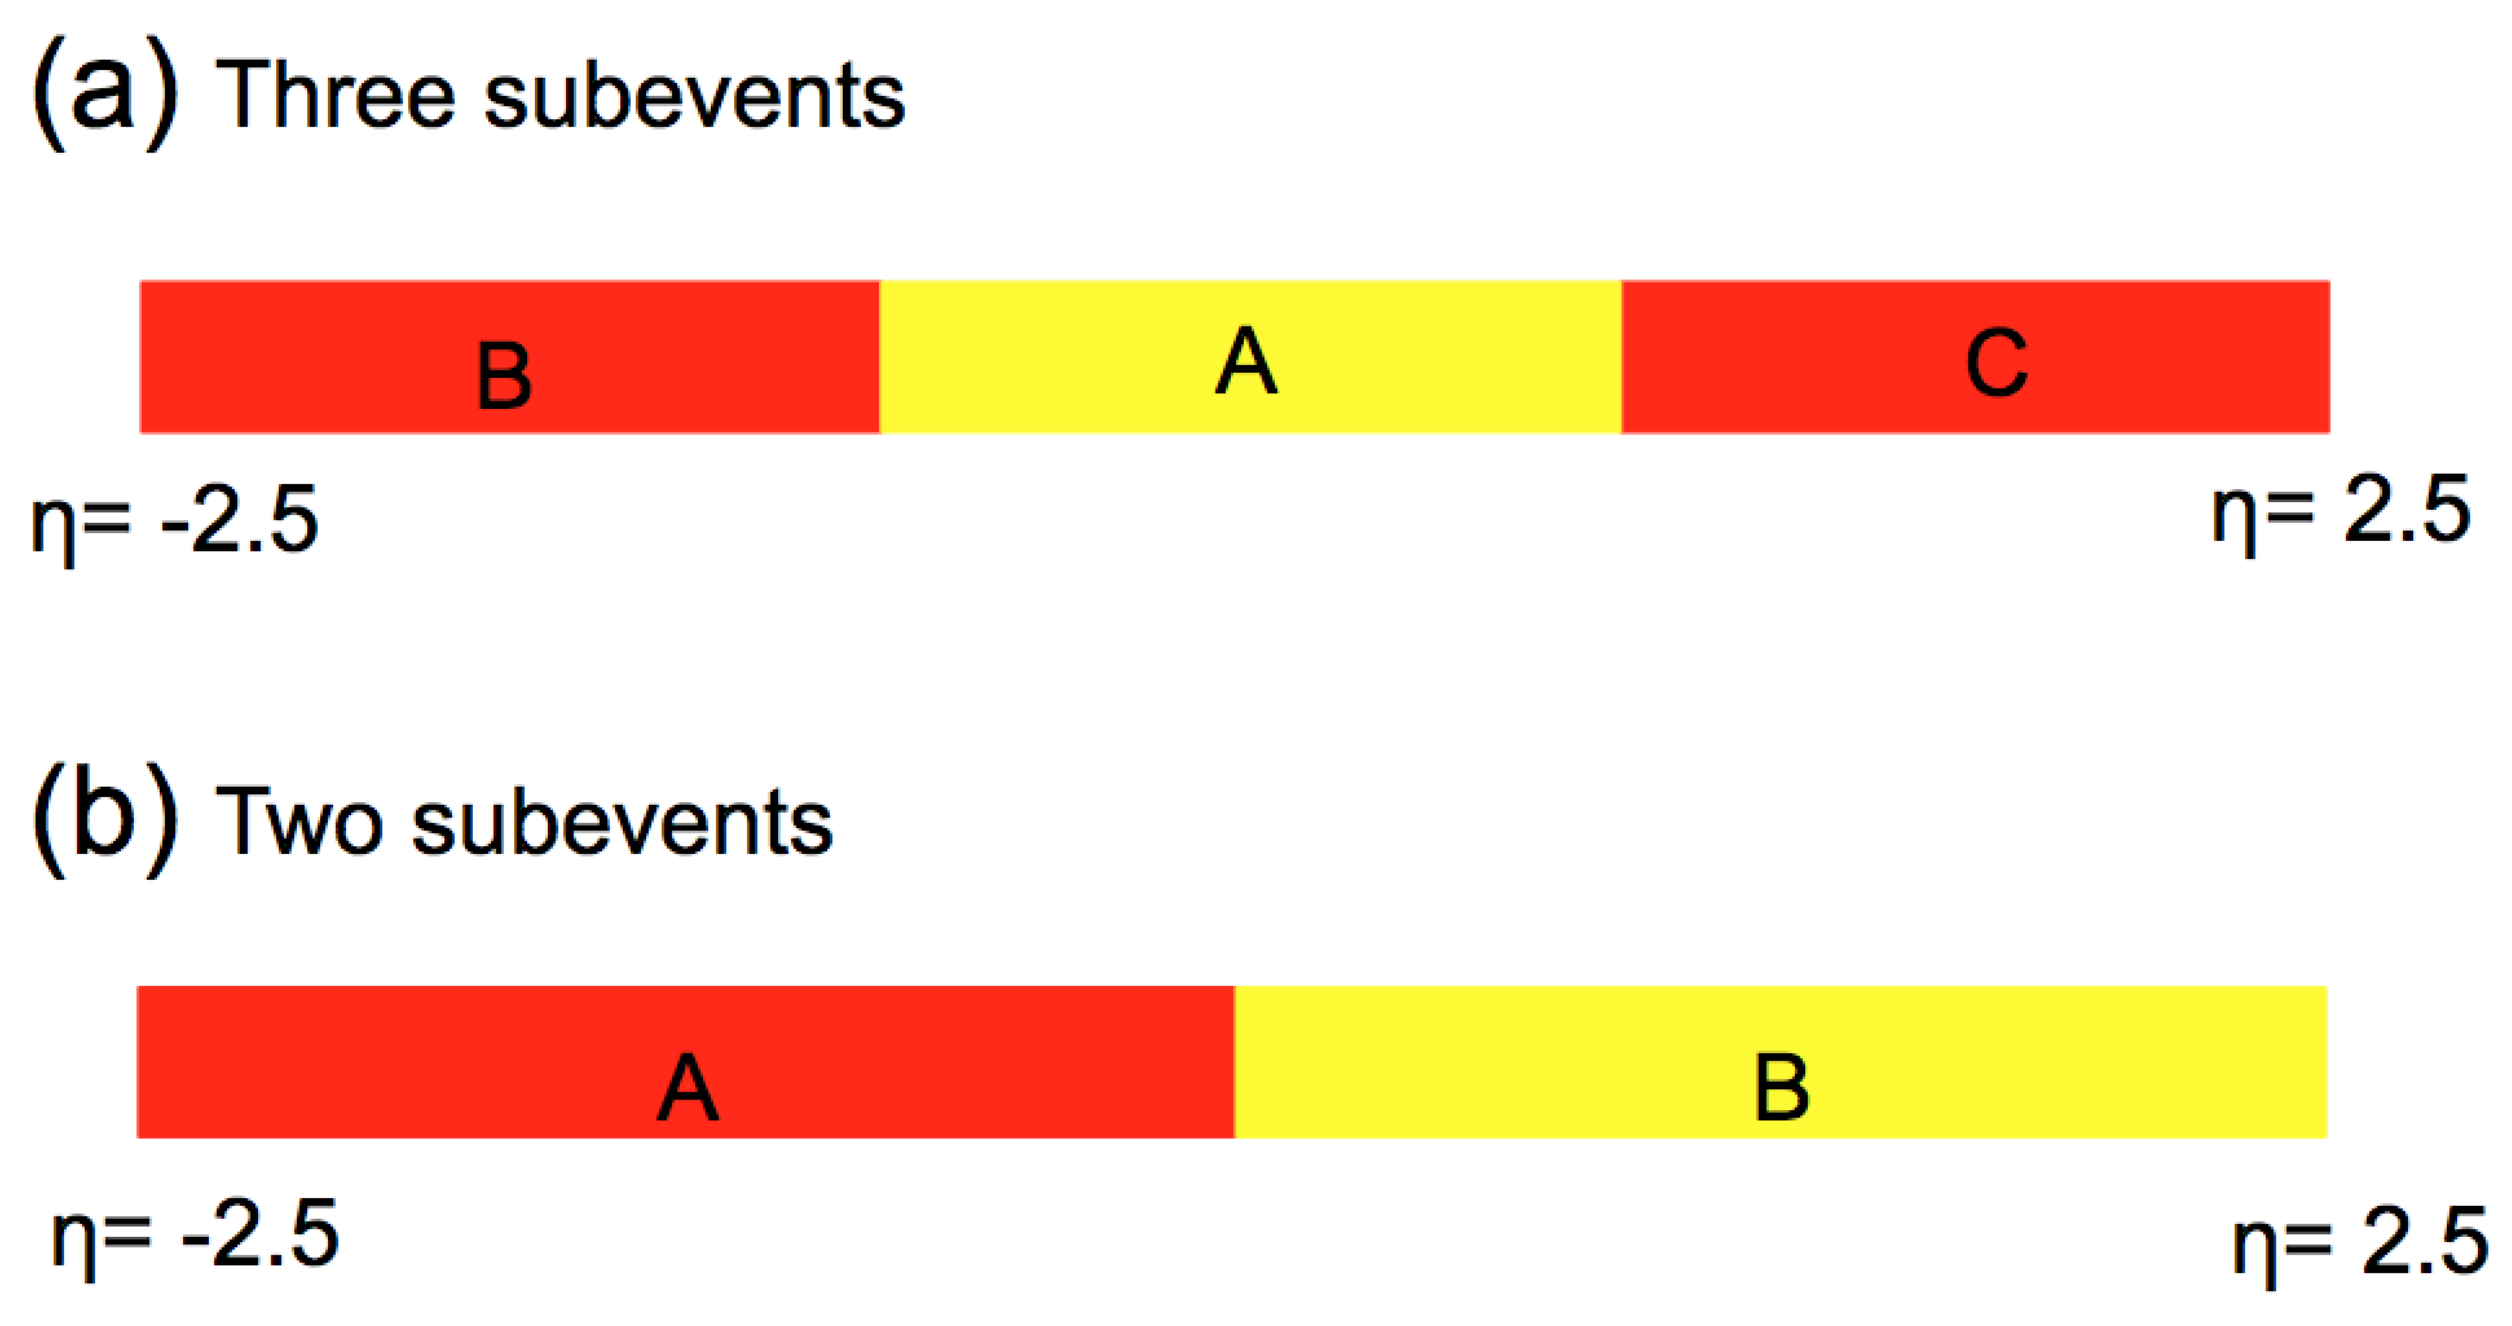
\includegraphics[width=0.7\columnwidth]{figs/sec_mtd/subevt_demo.png}
\caption{The $\eta$ ranges for the subevents in three-subevent method (a) and two-subevent method (b).}
\label{fig:subevt_demo}
\end{figure}

In this section, we will quickly go over all the formulas used for the analysis. Detailed descriptions will be discussed in the reference method paper~\cite{jjia}.

\subsection{Traditional cumulant}
Compared with newly developed subevent cumulant, the existing cumulant method is referred as traditional cumulant, where the 4-particle cumulant is defined as:
\begin{equation}
C_{n}\{4\}\equiv \lr{4}-2\lr{2}^{2}
\end{equation}
Using the direct or Q-cumulant technique, 4-particle correlation $\lr{4}$ and 2-particle correlation $\lr{2}$ are defined as~\cite{Bilandzic:2010jr, Bilandzic:2013kga}:
\begin{equation}
\begin{split}
\lr{2}&\equiv \frac{|Q_{n}|^{2}-M}{M(M-1)} \\
\lr{4}&\equiv \frac{|Q_{n}|^{4}+|Q_{2n}|^{2}-2\text{Re}(Q_{2n}Q_{n}^{*}Q_{n}^{*})-4(M-2)|Q_{n}|^{2}+2M(M-3)}{M(M-1)(M-2)(M-3)}
\end{split}
\end{equation}
where $M$ is the multiplicity in each event and $Q_{n}$ is calculated event-by-event:
\begin{equation}
Q_{n}\equiv\sum_{i}e^{in\phi_{i}}
\end{equation}
and without special mention, in this analysis, only the real part of the inner products (e.g. $Q_{2n}^{2}-2Q_{2n}Q_{n}^{*}Q_{n}^{*}$) is taken.



\subsection{2 sub-event method}
The cumulant is defined in a way that the non-flow sources associated with lower number of particles will be subtracted. Since in the framework of sub-event cumulant, the way non-flow sources are correlated is changed, the corresponding cumulant definition also needs to be changed:
\begin{equation}
C_{n}^{a,a|b,b}\{4\}\equiv \lr{4}_{a.a|b,b}-2\lr{2}_{a|b}^{2}
\end{equation}
where subscript $a,a|b,b$ defines how the four particles are arranged in the two sub-events. In this type, particles in the same sub-events are always correlated with particles in the other sub-events. In other words, particles in the same sub-events will not be correlated with each other, so that the short-range non-flow sources are suppressed. There will be an alternative arrangement for 2 sub-event cumulant: $a,b|a,b$. In this analysis, we will only discuss the first type $a,a|b,b$ since there are less residual non-flow contribution compared with the other type.

Following similar direct cumulant technique, 4-particle correlation $\lr{4}_{a,a|b,b}$ and 2-particle correlation $\lr{2}_{a|b}$ can be calculated in a single event loop:
\begin{equation}
\begin{split}
\lr{2}_{a|b}&\equiv \frac{Q_{n,a}Q_{n,b}}{M_{a}M_{b}} \\
\lr{4}_{a,a|b,b}&\equiv \frac{(Q_{n,a}^{2}-Q_{2n,a})(Q_{n,b}^{2}-Q_{2n,b})^{*}}{M_{a}(M_{a}-1)M_{b}(M_{b}-1)}
\end{split}
\end{equation}
where $M_{a}$ and $M_{b}$ are number of particles in each sub-event. $Q_{n,a}$ and $Q_{n,b}$ are the Q-vector in each sub-event, where the definition is same as the traditional cumulant.



\subsection{3 sub-event method}
Similar as the 2 sub-event method, depending on how the particles are correlated between sub-events, there are two types for the cumulant definition: $C_{n}^{a,a|b,c}\{4\}$ and $C_{n}^{a,b|a,c}\{4\}$. For the same reason as 2 sub-event method, we only consider the first type, where there is no correlation within the sub-event. The definition of the 4-particle 3 sub-event cumulant $C_{n}^{a,b|a,c}$ is:
\begin{equation}
C_{n}^{a,a|b,c}\{4\} \equiv \lr{4}_{a,a|b,c}-2\lr{2}_{a|b}\lr{2}_{a|c}
\end{equation}
where subscript $a,b|a,c$ defines how the four particles are arranged in the two sub-events: 2 particles from sub-event A and the other two from B and C separately. It is worth mentioning that there are two unique combinations by rotating the sub-event A, B and C, which will contribute to the total number of pairs.

Similarly, 4-particle correlation $\lr{4}_{a,a|b,c}$ and 2-particle correlation $\lr{2}_{a|b}$ and $\lr{2}_{a|c}$ can be calculated using the direct cumulant technique:
\begin{equation}
\begin{split}
\lr{2}_{a|b}&\equiv \frac{Q_{n,a}Q_{n,b}}{M_{a}M_{b}} \\
\lr{2}_{a|c}&\equiv \frac{Q_{n,a}Q_{n,c}}{M_{a}M_{c}} \\
\lr{4}_{a,a|b,c}&\equiv \frac{(Q_{n,a}^{2}-Q_{2n,a})Q_{n,b}^{*}Q_{n,c}^{*}}{M_{a}(M_{a}-1)M_{b}M_{c}}
\end{split}
\end{equation}
where the definitions are the same as 2 sub-event method.

All the formulas in this section are without particles weights. The formulas with particle weights (tracking efficiency and detector effects) will be introduced in the following section~\cite{Abelev:2014mda}. In this analysis, we will only focus on the 4-particle cumulant. One reason is that due to the large statistical errors, it is not practical to measure 6-particle cumulant in small systems like $pp$. But the main reason is that traditional cumulant relies on correlation of more particles to suppress the non-flow sources, since non-flow source is usually associated with few particles. However, this is not true for sub-event method. By purposely put the particles into sub-events extended in a wide $\eta$ range, the non-flow correlation is already suppressed. In other word, the advantage of sub-event method is to suppress the non-flow without involving more particles. For these reasons, we will only discuss the results of 4-particle cumulants in this note. 



